
\chapter{Random Vectors}

In this chapter, we assume that a probability space $(S, \mathcal{A}, P)$ is given.

\section{Bivariate Distributions}
Given two random variables $X$ and $Y$ defined on the probability space $(S, \mathcal{A} , P )$, we can think of them acting together as a random vector $(X, Y)$ taking values in $\mR^2$. 

\begin{example}
Let $S = \{ \epsdice{1} , \epsdice{2} , \epsdice{3} , \epsdice{4} , \epsdice{5} , \epsdice{6} \}$ with $\mathcal{A} = \mathcal{P} (S)$ be the probability space associated to throwing a fair dice. Assume that we throw two such die and consider the following random variable:
\begin{enumerate}[label=\arabic*)]
    \item $X$: ``The number of dots on the first dice''.
    \item $Y$: ``The number of dots on the second dice''.
\end{enumerate}
Assuming the two dice are independent, what is the probability that $X \leq 2$ and $Y \leq 2$?
\end{example}

\begin{sol*}
Denote this probability by $p$. There is $1/6$ chance of obtaining all the different faces. If $A = \{ X \leq 2 \} \cap \{ Y \leq 2 \}$, then
    \begin{align*}
        p &= P (A) \\ 
        &= P (X = 1, Y = 1) + P (X = 1, Y = 2) + P (X = 2, Y = 1) + P (X = 2, Y = 2) \\ 
        &= \frac{1}{36} + \frac{1}{36} + \frac{1}{36} + \frac{1}{36} \\ 
        &= \frac{4}{36} = \frac{1}{9} .
    \end{align*}
We denote $p$ by $F_{X, Y} (2, 2)$ and this is called the joint distribution function of $X$ and $Y$ at $ (X, Y) = (2, 2)$. \hfill $\triangle$
\end{sol*}

\textbf{Notations:}
    \begin{itemize}
        \item the set $\{ s \, : \, X (s) \leq x , Y (s) \leq y \} = \{ X \leq x \} \cap \{ Y \leq y \}$ will be denoted by $\{ X \leq x , Y \leq y \}$.
        \item the probability of $\{ X \leq x , Y \leq y \}$ is denoted by $P (X \leq x , Y \leq y )$. 
    \end{itemize}

\begin{definition}
The \underline{joint distribution function} of a pair of random variables $X$, $Y$ is the mapping $F_{X, Y} : \mR^2 \ra [0, 1]$ given by
    \[
        F_{X, Y} (x, y) = P (X \leq x , Y \leq y ) .
    \]
\end{definition}

\underline{Basic Properties:}
    \begin{enumerate}[label=\arabic*)]
        \item $\displaystyle \lim_{x \ra -\infty} \lim_{y \ra -\infty} F_{X, Y} (x, y) = \lim_{y \ra -\infty} \lim_{x \ra -\infty} F_{X, Y} (x, y) = 0$.
        \item $\displaystyle\lim_{x \ra \infty} \lim_{y \ra \infty} F_{X, Y} (x, y) = \lim_{y \ra \infty} \lim_{x \ra \infty} F_{X, Y} (x, y) = 1$.
        \item Increasing: $F(x_1, y_1) \leq F(x_2, y_2)$, for any $x_1 \leq x_2$ and $y_1 \leq y_2$.
        \item\label{P:MarginalInX}$F_X (x) = \displaystyle \lim_{y \ra \infty} F_{X, Y} (x, y)$. [Proof: Notice that $\{ Y < \infty \} = S$, so that
        \[
            F_X (x) = P (X \leq x ) = P (X \leq x , Y < \infty ) = \lim_{y \ra \infty} F_{X, Y} (x, y) .]
        \]
        \item\label{P:MarginalInY} $F_Y (y) = \displaystyle \lim_{x \ra \infty} F_{X, Y} (x, y)$.
    \end{enumerate}

\begin{definition}
If $X$ and $Y$ are random variables, then the above limits in items 4 and 5 are called the \underline{marginal distributions} of the random vector $(X, Y)$.
\end{definition}

\begin{example}
Assume that $X$ and $Y$ are random variables with joint distribution function
    \[
        F_{X, Y} = \left\lbrace \begin{matrix} 1 - e^{-x} - e^{-y} + e^{-x-y} & \text{if } x, y \geq 0 .\\
        0 & \text{otherwise.} \end{matrix} \right. 
    \]
Find the marginals of this joint distribution.
\end{example}

\begin{sol*}
We first let $y \ra \infty$, so that, if $x \geq 0$, then 
    \[
        \lim_{y \ra \infty} F_{X, Y} (x, y) = \lim_{y \ra \infty} 1 - e^{-x} - e^{-y} + e^{-x - y} = 1 - e^{-x} .
    \]
When $x < 0$, then $F_{X, Y} (x, y) = 0$. Therefore, this gives us $F_X (x) = \max \{ 0 , 1 - e^{-x} \}$, which is the distribution function of the exponential distribution with parameter $\lambda = 1$. Similarly, $F_Y (y) = \max\{ 0, 1 - e^{-y} \}$. \hfill $\triangle$
\end{sol*}

Notice that, in the last example, 
    \[
        F_{X, Y} (x, y) = F_X (x) F_Y (y)
    \]
meaning that
    \[
        P (X \leq x , Y \leq y) = P (X \leq x) P (Y \leq y) .
    \]
When this happens, we say that $X$ and $Y$ are independent.

\begin{definition}
Let $X$ and $Y$ be two random variables with joint distribution function $F_{X, Y}$. Then $X$ and $Y$ are \underline{independent} if for every $x, y \in \mR$,
    \[
        F_{X, Y} (x, y) = F_X (x) F_Y (y)    \]
where $F_X$ and $F_Y$ are the marginals of $X$ and $Y$ respectively.
\end{definition}

\underline{\textbf{Remark.}} When $X$ and $Y$ are not independent, we say that they are \underline{dependent}.

\section{Continuous Random Vectors}

\begin{definition}
Two random variables $X$, $Y$ are \underline{(jointly) continuous} if there is an integrable function $f : \mR \times \mR \ra [0, \infty )$ such that
    \[
        F_{X, Y} (x, y) = \iint_{R} f(u, v) \, dA \,
    \]
for every $x, y \in \mR$, where $R = (-\infty , x] \times (-\infty , y]$.
\end{definition}

\underline{\textbf{Remark:}} 
    \begin{itemize}
    \item When $X$ and $Y$ are jointly continuous, the function $f(x, y)$ in the integral is usually called the \underline{joint probability density function} and usually denoted by $f_{X, Y}$. 
    \item Recall from multivariable calculus that, in cartesian coordinates,
        \[
            \iint_R f (u, v) \, dA  = \int_{-\infty}^x \int_{-\infty}^y f(u, v) \, dv du .
        \]
    \item What we mean by an integrable function is a function $f : \mR \times \mR \ra [0, \infty )$ such that
        \[
            \int_{-\infty}^\infty \int_{-\infty}^\infty f (x, y) \, dx dy < \infty .
        \]
    \end{itemize}

\begin{example}\label{Ex:JointDensityRadioactiveParticle}
Suppose that a radioactive particle is randomly located in a square with sides of unit length. That is, if two regions within the unit square and of equal area are considered, the particle is equally likely to be in either region. Let $X$ and $Y$ denote the coordinates of the particle's location. A reasonable model for the joint probability density function of $X$ and $Y$ is
    \[
        f_{X, Y} (x, y) = \left\lbrace \begin{matrix} 1 & \text{if } (x, y) \in [0, 1] \times [0, 1] \\
        0 & \text{elsewhere.} \end{matrix} \right.
    \]
\begin{enumerate}[label=\alph*)]
    \item Sketch the probability density function.
    \item Find $F(0.2, 0.4)$.
    \item\label{Ex:PartcOfRadioActiveParticle} Find $P (0.1 \leq X \leq 0.3 , 0 \leq Y \leq 0.5)$.
    \item Find $P (X + Y \leq 0.5 )$.
\end{enumerate}
\end{example}

\begin{sol*}
\begin{enumerate}[label=\alph*)]
\item Using Desmos 3D online app, the joint density function looks like this:
    \begin{figure}[ht]
    \centering 
    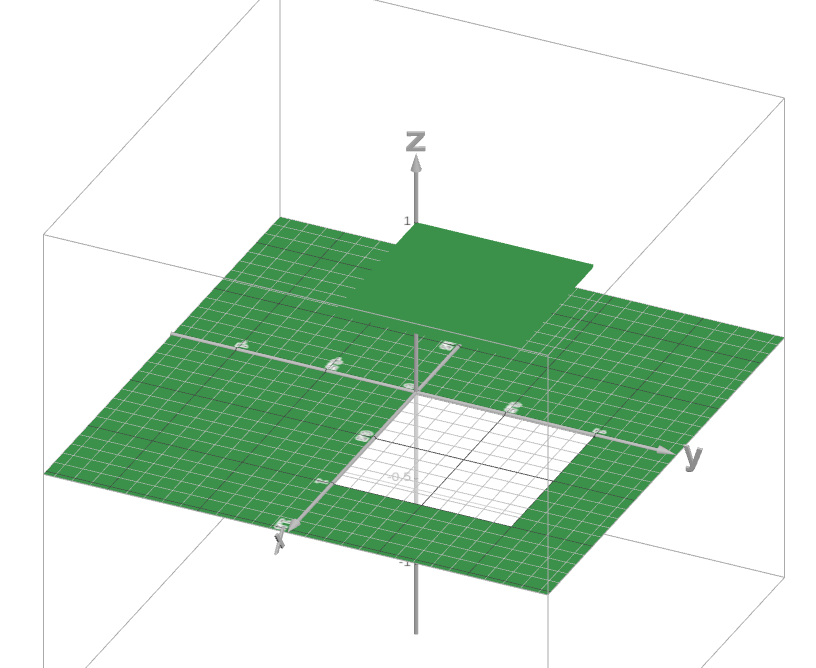
\includegraphics[scale=0.2]{JointDistributionChapE.png}
    \end{figure}
\item By definition, we have
    \[
        F(0.2, 0.4) = \iint_R f_{X, Y} (u, v) \, dA ,
    \]
where $R = (-\infty , x ] \times (-\infty , y]$. Since the function is $0$ outside $[0, 1] \times [0, 1]$, we can restrict the integral to $R \cap [0, 1] \times [0, 1] = [0, 0.2] \times [0, 0.4]$. Therefore
    \[
        F(0.2, 0.4) = \int_{0}^{0.4} \int_0^{0.2} 1 \, dx dy = (0.4) (0.2) = 0.08 .
    \]
\item Here, we will use the fact that $\{ 0.1 \leq X \leq 0.3, 0 \leq Y \leq 0.5 \}$ is equal to
    \[
        \{ X \leq 0.3 , Y \leq 0.5 \} \cap \overline{\{ X \leq 0.1 , Y \leq 0.5 \} \cup \{ X \leq 0.3 , Y \leq 0 \}}.
    \]
Using the identity $P (A \cap \overline{B}) = P (A) - P (B)$, when $B \subset A$ and with $A = \{ X \leq 0.3, Y \leq 0.5 \}$ and $B = \{ X \leq 0.1 , Y \leq 0.5\} \cup \{ X \leq 0.3 , Y \leq 0 \}$, we find that
    \[
        P (0.1 \leq X \leq 0.3 , 0 \leq Y \leq 0.5) = P (A) - P (B) .
    \]
Using the fact that $P (C \cup D) = P (C) + P (D) - P (C \cap D)$, with $C = \{ X \leq 0.1 , Y \leq 0.5 \}$ and $D = \{ X \leq 0.3 , Y \leq 0 \}$, we find that
    \[
        P (B) = P (X \leq 0.1 , Y \leq 0.5) + P (X \leq 0.3 , Y \leq 0 ) - P (X \leq 0.1, Y \leq 0) .
    \]
Combining everything together, we get
    \begin{align*}
        P (0.1 \leq X \leq 0.3 , 0 \leq Y \leq 0.5 ) &= P (X \leq 0.3, Y \leq 0.5) - P (X \leq 0.1 , Y \leq 0.5) \\
        & \quad - P (X \leq 0.3 , Y \leq 0 ) + P (X \leq 0.1, Y \leq 0) \\ 
        & = F (0.3, 0.5) - F (0.1, 0.5) - F(0.3, 0) + F (0.1, 0) \\ 
        &= \int_{0.1}^{0.3} \int_{0}^{0.5} 1 \, dy dx = (0.2)(0.5) = 0.1 .
    \end{align*}
    \item Let $R = \{ (X, Y) \, : \, X + Y \leq 0.5 \}$. Then, because $f_{X, Y} = 0$ outside of $[0, 1] \times [0, 1]$, we can write the region as
        \[
            R = \{ (X, Y) \, : \, 0 \leq X \leq 0.5 , 0 \leq Y \leq 0.5 - X \} .
        \]
    Therefore, we get
        \begin{align*}
            P ( (X, Y) \in R ) = P (0 \leq X \leq 0.5, 0 \leq Y \leq 0.5 - X ) &= \int_0^{0.5} \int_0^{0.5 - x} 1 \, dy dx \\
            &= \int_0^{0.5} (0.5 - x) \, dx = 0.025 .
        \end{align*}
    Notice that 
        \[
            P ( (X, Y) \in R ) = \iint_R f_{X, Y} (x, y) \, dA . \tag*{$\triangle$}
        \]
    
\end{enumerate}
\end{sol*}

\underline{\textbf{Remark:}} 
\begin{itemize}
    \item If $R = [x_0, y_0] \times [x_1 , y_1]$ is a rectangle in the plane, then
    \[
        P ( (X, Y) \in R ) = P (x_0 \leq X \leq x_1 , y_0 \leq Y \leq y_1) = \iint_R f (u, v) \, dA .
    \]
    \item More generally, if $R$ is any region in the plane, then
    \[
        P ( (X, Y) \in R ) = \iint_R f (u, v) \, dA .
    \]
    \item When $(X, Y)$ are jointly continuous with density $F_{X, Y}$, then we can recover the joint probability mass function $f_{X, Y}$ in the following way:
        \[
            f_{X, Y} (x, y) = \frac{\partial^2}{\partial x \partial y} F (x, y) .
        \]
    \item The density functions of $X$ and $Y$ can be recovered in the following ways:
        \begin{enumerate}[label=\arabic*)]
            \item $f_X (x) = \displaystyle\int_{-\infty}^\infty f_{X, Y} (x, y) \, dy$;
            \item $f_Y (y) = \displaystyle\int_{-\infty}^\infty f_{X, Y} (x, y) \, dx$.
        \end{enumerate}
\end{itemize}

\section{Marginals and Independence}

\begin{example}
Let $(X, Y)$ be a random vector with probability density function
    \[
        f_{X, Y} (x, y) = \left\lbrace \begin{matrix} 2 x & \text{ if } (x, y) \in [0, 1] \times [0, 1] \\
        0 & \text{elsewhere.} \end{matrix} \right.
    \]
\begin{enumerate}[label=\alph*)]
    \item Sketch $f_{X, Y}$.
    \item Find the marginals of $X$ and $Y$.
    \item What can you conclude on $f_{X, Y}$?
\end{enumerate}
\end{example}

\begin{sol*}
\begin{enumerate}[label=\alph*)]
    \item The graph of the function should look like this:
        \begin{figure}[ht]
        \centering 
        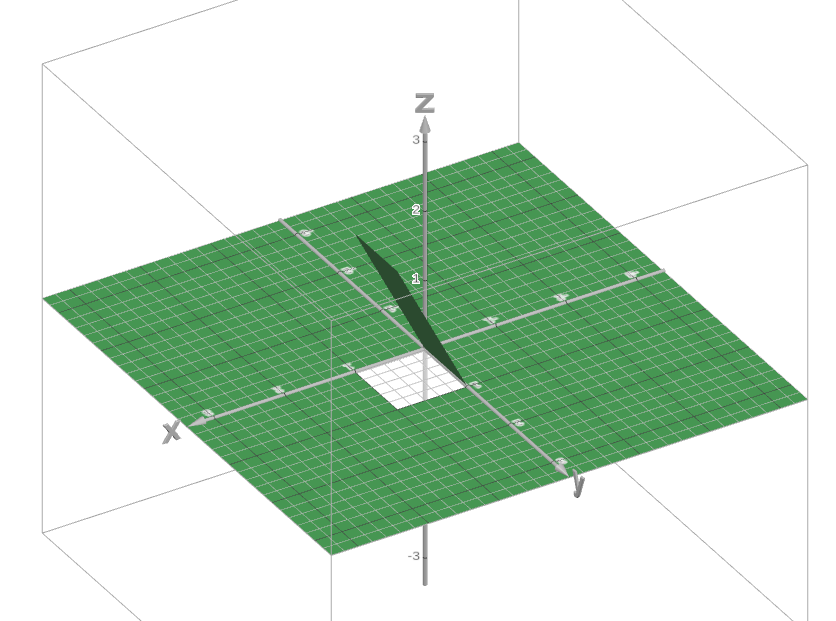
\includegraphics[scale=0.2]{MarginalIndependenceGraphChapE.png}
        \end{figure}
    \item By definition $F_X (x) = \lim_{y \ra \infty} F_{X, Y} (x, y)$. Since $X$ and $Y$ are jointly continuous, we have
        \[
            F_X (x) = \lim_{y \ra \infty} \int_{-\infty}^x \int_{-\infty}^y f_{X, Y} (u, v) \, dv du .
        \]
    When $x < 0$, we have $F_X (x) = 0$. For $0 \leq x \leq 1$, we have $f_{X, Y} (x) = 2x$, if $y$ is big enough, so that
        \[
            F_X (x) = \int_{0}^x \int_0^1 2u \, dv du = x^2 .
        \]
    When $x > 1$ and $y$ is sufficiently big (in fact bigger than $1$), we see that $F_X (x) = 1$. Therefore, 
    $$
        F_X (x) = \left\lbrace \begin{matrix} 0 & x < 0 \\ x^2 & 0 \leq x \leq 1 \\ 1 & x > 1 \end{matrix} \right.
    $$
    or we can also rewrite $F_X (x) = \big( \max \{ 0, \min \{ x , 1 \} \} \big)^2$. 

    With similar calculations, we obtain
        $$ 
            F_Y (y) = \left\lbrace \begin{matrix} 0 & y < 0 \\ x & 0 \leq y \leq 1 \\ 1 & y > 1 \end{matrix} \right. 
        $$ 
    or we can write $F_Y (y) = \max \{ 0 , \min \{ y, 1 \} \}$. 
    \item Recall that $f_X = \frac{d}{dx} F_X$. Therefore, when $x < 0$ and $x > 1$, we have $f_X = 0$. When $0 < x < 1$, we have $f_X (x) = 2x$. Similarly, we have $f_Y = \frac{d}{dy} F_Y$. Therefore, when $y < 0$ and $y > 1$, we have $f_Y = 0$. When $0 < y < 1$, we have $f_Y (y) = 1$. Remarkably, we get
        \[
            f_{X, Y} (x, y) = f_X (x) f_Y (y) !! \tag*{$\triangle$}
        \]
\end{enumerate}
\end{sol*}

\begin{theorem}
Jointly continuous random variables $X$ and $Y$ are independent if and only if there are two functions $g, h : \mR \ra [0 , \infty )$ such that
    \[
        f_{X, Y} (x, y) = g(x) h(y) \quad \forall x, y \in \mR .
    \]
\end{theorem}

\underline{\textbf{Remark:}} 
    \begin{itemize}
        \item The functions $g$ and $h$ are called the \underline{marginal probability density functions} of the random vector $(X, Y)$. 
        \item The function $g$ is equal to $f_X$, the probability density function of $X$.
        \item The function $h$ is equal to $f_Y$, the probability density function of $Y$.
    \end{itemize}

%\begin{example}
%Assume that $X$ and $Y$ are random variables with joint distribution function
%    \[
%        F_{X, Y} (x, y) = \left\lbrace \begin{matrix} 1 - e^{-x} - e^{-y} + e^{-x-y} & \text{if } x, y \geq 0 \\
%        0 & \text{elsewhere} \end{matrix} \right.
%    \]
%\begin{enumerate}[label=\alph*)]
%    \item Find the joint probability density function of $X$ and $Y$.
%    \item Are $X$ and $Y$ independent?
%\end{enumerate}
%\end{example}

%\begin{sol*}

%\end{sol*}

\begin{example}\label{Example:NonIndependence}
Let $X$ and $Y$ be two random variables having joint probability density function
    \[
        f_{X, Y} (x, y) = \left\lbrace \begin{matrix} 2 e^{-x - y} & \text{if } 0 < x < y \\
        0 & \text{elsewhere.} \end{matrix} \right. 
    \]
Are $X$ and $Y$ independent?
\end{example}

\begin{sol*}
The marginal density function of $X$ is given by
    \[
        f_X (x) = \int_{-\infty}^\infty f_{X, Y} (x, y) \, dy .
    \]
When $x < 0$, then $f_{X, Y} (x, y) = 0$ and so $f_X (x) = 0$. Let $x > 0$. Then, $f_{X, Y} (x, y) = 2 e^{-x - y}$ when $y > x$ and
    \[
        f_X (x) = \int_x^\infty 2e^{-x - y} \, dy = 2e^{-2x} .
    \]
Thus, $f_X (x) = 0$ if $x < 0$ and $f_X (x) = 2e^{-2x}$, if $x \geq 0$. 

The marginal density function of $Y$ is given by
    \[
        f_Y (y) = \int_{-\infty}^\infty f_{X, Y} (x, y) \, dx .
    \]
When $y < 0$, then $f_{X, Y} (x, y) = 0$ and so $f_Y (y) = 0$. Let $y > 0$. Then $f_{X, Y} (x, y) = 2e^{-x - y}$ when $0 < x < y$, so that
    \[
        f_Y (y) = \int_0^y 2e^{-x - y} \, dy = 2e^{-y} (1 - e^{-y} ) .
    \]
Therefore, $f_Y (y) = 0$ when $y < 0$ and $f_Y (y) = 2e^{-y} (1 - e^{-y})$ when $y \geq 0$. 

We see that
    \[
        f_{X, Y} (x, y) \neq f_X (x) f_Y (y)
    \]
and therefore, $X$ and $Y$ are not independent. \hfill $\triangle$
\end{sol*}

\subsubsection*{Conditional Density Functions}
When we don't have any information on $X$, the marginal density function $f_Y$ of $Y$ is the average
    \[
        f_Y (y) = \int_{-\infty}^\infty f_{X, Y} (x, y) \, dx .
    \]
But, if we have information on values of $X$, we may consider $P (Y \leq y | X = x)$. However, since $P (X = x) = 0$ in the continuous case, we can't use formula $P (A|B) = P (A \cap B)/ P(B)$ to get an expression of this probability. Instead, we compute $P (Y \leq y | x \leq X \leq X + \Delta x )$, for a small $\Delta x$ and then divide by $\Delta x$. Doing so, we get that
    \begin{align*}
        F_{Y | X = x} (y) = \lim_{\Delta x \ra 0 } P (Y \leq y | x \leq X \leq x + \Delta x ) &= \lim_{\Delta x \ra 0} \frac{P (Y \leq y , x \leq X \leq x + \Delta x)}{P (x \leq X \leq x + \Delta x )} \\
        &= \lim_{\Delta x \ra 0} \frac{\int_{-\infty}^y \frac{1}{\Delta x}\int_{x}^{x + \Delta x} f_{X, Y} (u, v) \, du dv}{ \frac{1}{\Delta x}\int_x^{x + \Delta x} f_X (u) \, du} \\
        &= \int_{-\infty}^y \frac{f_{X, Y} (x, v)}{f_X (x)} \, dv .
    \end{align*}

\begin{definition}
If $X$ and $Y$ are jointly continuous random variables, then the \ul{conditional density function of $Y$ given that $X = x$} is denoted by $f_{Y|X} (\cdot | x)$ and is defined by
    \[
        f_{Y|X} (y|x) = \frac{f_{X, Y} (x, y)}{f_X (x)}
    \]
for any $y \in \mR$ and $x$ satisfying $f_X (x) > 0$. 
\end{definition}

\underline{\textbf{Remark:}} 
\begin{itemize}
    \item In the continuous case, we define
        \[
            P (Y \leq y | X = x) := \int_{-\infty}^y f_{Y|X} (v|x) \, dv .
        \]
    \item Similarly, conditioning with respect to the event $\{ Y = y \}$, then the conditional density function of $X$ given that $Y = y$ is
        \[
            f_{X|Y} (x|y) = \frac{f_{X, Y} (x, y)}{f_Y (x)} .
        \]
    \item The formulas of the conditional density are very similar to the definition of $P (A|B)$.
\end{itemize}

\begin{example}
Find $f_{X|Y}$ if $X$ and $Y$ have joint probability density function 
    \[
        f_{X, Y} (x ,y) = \left\lbrace \begin{matrix} 2 e^{-x - y} & \text{ if } 0 < x < y < \infty \\
        0 & \text{otherwise.} \end{matrix} \right.
    \]
\end{example}
\begin{sol*}
From Example \ref{Example:NonIndependence}, the density of $Y$ is
    \[
        f_Y (x) = \int_{-\infty}^\infty f_{X, Y} (x, y) \, dx = 2e^{-y} (1 - e^{-y}) .
    \]

For $y < 0$, we have $f_{X|Y} (x|y) = 0$. For $y > 0$, we have
    \[
        f_{X|Y} (x|y) = \frac{2e^{-x-y}}{2e^{-y} (1 - e^{-y})} = \frac{e^{-x}}{1 - e^{-y}} . \tag*{$\triangle$}
    \]
\end{sol*}

\section{Important Measurements}

Expectation is defined for a random variable. Therefore, we will compute the expectation of a random variable $Z = g (X, Y)$, that is
    \[
        Z (s) = g (X (s), Y (s)) \quad (s \in S ),
    \]
for some function $g : \mR \times \mR \ra \mR$.

\begin{example}
Compute the expected value of the random variable $Z = X + Y$, if $X$ and $Y$ have joint probability density function $f_{X, Y}$.
\end{example}

\begin{sol*}
By definition, the expectation of $Z$ is
    \[
        \mathrm{Exp} (Z) = \int_{-\infty}^\infty z f_Z (z) \, dz .
    \]
However, we have
    \[
        P (Z \leq z ) = P (X + Y \leq z) = \iint_A f_{X, Y} (x, y) \, dA
    \]
where $A = \{ (x, y) \, : \, x + y \leq z \}$. We therefore see that
    \[
        F_Z (z) = \int_{-\infty}^\infty \int_{-\infty}^{z - x} f_{X, Y} (x, y) \, dy dx = \int_{-\infty}^z \int_{-\infty}^\infty f_{X, Y} (u, v-u) \, du dv
    \]
after the transformation $u = x$ and $v = x + y$. Therefore, differentiating, we obtain
    \[
        f_Z (z) = \int_{-\infty}^\infty f_{X, Y} (u, z - u ) \, du .
    \]
Replacing in the formula of the expectation, we find that
    \[
        \mathrm{Exp} (Z) = \int_{-\infty}^\infty z \int_{-\infty}^\infty f_{X, Y} (u, z - u) \, du dz = \int_{-\infty}^\infty \int_{-\infty}^\infty z f_{X, Y} (u, z - u ) \, du dz . 
    \]
Now, reset $u = x$ and $y = z - u$, so that $z = x + y$ and therefore
    \[
        \mathrm{Exp} (Z) = \int_{-\infty}^\infty \int_{-\infty}^\infty (x + y) f_{X, Y} (x, y) \, dx dy . \tag*{$\triangle$} .
    \]
\end{sol*}

\begin{theorem}
If $X$ and $Y$ are random variables that are jointly continuous and if $Z = g (X, Y)$ is a continuous random variable for some function $g : \mR \times \mR \ra \mR$, then
    \[
        \mathrm{Exp} (Z) = \int_{-\infty}^\infty \int_{-\infty}^\infty g (x, y) f_{X, Y} (x, y) \, dx dy 
    \]
whenever this integral exists.
\end{theorem}

\underline{\textbf{Properties:}}
    \begin{itemize}
        \item $\mathrm{Exp} (a X + bY) = a \mathrm{Exp} (X) + b \mathrm{Exp} (Y)$.
        \item If $X$ and $Y$ are independent random variable, then
            \[
                \mathrm{Exp} (X Y) = \mathrm{Exp} (X) \mathrm{Exp} (Y) .
            \]
    \end{itemize}

\begin{example}
Let $X, Y$ be two uniformly distributed on the unit disc, so that
    \[
        f_{X, Y} (x, y) = \left\lbrace \begin{matrix} \pi^{-1} & \text{if } x^2 + y^2 \leq 1 \\
        0 & \text{otherwise} \end{matrix} \right.
    \]
Find $\mathrm{Exp} (\sqrt{X^2 + Y^2})$.
\end{example}

\begin{sol*}
Here, $Z = \sqrt{X^2 + Y^2}$, so that $g (x, y) = \sqrt{x^2 + y^2}$. Applying the formula of the expectation, we find
    \[
        \mathrm{Exp} (Z) = \int_{-\infty}^\infty \int_{-\infty}^\infty \sqrt{x^2 + y^2} f_{X, Y} (x, y) \, dx dy .
    \]
Since $f_{X, Y} (x, y) = 0$ when $x^2 + y^2 > 1$, then
    \[
        \mathrm{Exp} (Z) = \iint_{D} \frac{\sqrt{x^2 + y^2}}{\pi} \, dA 
    \]
where $D = \{ (x, y) \, : \, x^2 + y^2 \leq 1 \}$. Using polar coordinates $x = r \cos \theta$ and $y = r \sin \theta$, we get
    \[
        \mathrm{Exp} (X) = \int_0^{2\pi} \int_0^1 \frac{r^3}{\pi} \, dr d\theta = \frac{1}{2} . \tag*{$\triangle$}
    \]
\end{sol*}

\subsection*{Covariance}

Recall that if $X$ and $Y$ are independent, then
    \[
        \mathrm{Exp} (XY) = \mathrm{Exp} (X) \mathrm{Exp} (Y) .
    \]
An interpretation of the last identity is that no information of $X$ and $Y$ mixed up the expectation of $XY$. We would like a measurement of how a random variable $X$ affects the outcome of another variable $Y$. In other words, we want to measure how $X$ and $Y$ are correlated!

\begin{definition}
The \underline{covariance} of the random variables $X$ and $Y$ is the quantity denoted $\mathrm{Cov} (X, Y)$ and given by
    \[
        \mathrm{Cov} (X, Y) = \mathrm{Exp} ( (X - \mu_X ) (Y - \mu_Y)),
    \]
where $\mu_X = \mathrm{Exp} (X)$ and $\mu_Y = \mathrm{Exp} (Y)$.
\end{definition}

\underline{\textbf{Remarks:}}
    \begin{itemize}
        \item The $\mathrm{Cov} (X, Y)$ depends upon the scale of measurement. This is why, in practice, we normalize to obtain the correlation (coefficient):
            \[
                \rho (X, Y) = \frac{\mathrm{Cov} (X, Y)}{\sigma_X \sigma_Y},
            \]
        where $\sigma_X = \sqrt{\mathrm{Var} (X)}$ and $\sigma_Y = \sqrt{\mathrm{Var} (Y)}$. In this case, $\rho \in [-1, 1]$. 
        \item When $\rho (X, Y) \neq 0$ it means there is a linear dependence between $X$ and $Y$, getting stronger as $\rho$ gets closer and closer to $-1$ or $1$. We have two different types of correlation between $X$ and $Y$:
            \begin{enumerate}[label=\arabic*)]
                \item $\rho (X, Y) > 0$, then when $X$ increases, then $Y$ increases.
                \item $\rho (X, Y) < 0$, then when $X$ increases, then $Y$ decreases.
            \end{enumerate}
    \end{itemize}

\begin{theorem}
If $X$ and $Y$ are random variables with means $\mu_X$ and $\mu_Y$, respectively, then
    \[
        \mathrm{Cov} (X, Y) = \mathrm{Exp} (XY) - \mathrm{Exp} (X) \mathrm{Exp} (Y) .
    \]
\end{theorem}

\begin{example}
Assume that $X$ and $Y$ are uniformly distributed on the triangle with vertices $(-1,0)$, $(0,1 )$, and $(1, 0)$. 
    \begin{enumerate}[label=\alph*)]
        \item Find $\mathrm{Cov} (X, Y)$.
        \item Are $X$ and $Y$ independent?
    \end{enumerate}
\end{example}

\begin{sol*}
    \begin{enumerate}[label=\alph*)]
        \item The joint density function of $X$ and $Y$ are
            \[
                f_{X, Y} (x, y) = \left\{ \begin{matrix} 1 & \text{ if } y-1 \leq x \leq 1 - y , \, 0 \leq y \leq 1 \\ 
                0 & \text{ elsewhere} \end{matrix} \right. 
            \]
        Using the formula for the expected value of the random variable $Z = XY$, we get
            \begin{align*}
                \mathrm{Exp} (XY) &= \int_{-\infty}^\infty \int_{-\infty}^\infty xy f_{X, Y} (x, y) \, dx dy \\ 
                &= \int_{0}^1 \int_{y-1}^{1-y} xy \, dxdy = 0 .
            \end{align*}
        After some calculations, we find that
            \[
                f_X (x) = \int_{-\infty}^\infty f_{X, Y} (x, y) \, dy = \left\lbrace \begin{matrix} 1 + x & \text{ if } -1 < x < 0 \\
                1 - x & \text{ if } 0 < x < 1 \\ 
                0 & \text{ elsewhere}
                \end{matrix} \right. 
            \]
        and
            \[
                f_Y (y) = \int_{-\infty}^\infty f_{X, Y} (x, y) \, dx = \left\lbrace \begin{matrix} 2 - 2y & \text{ if } 0 < y < 1 \\ 
                0 & \text{ elsewhere.} 
                \end{matrix} \right. 
            \]
        Therefore,
            \[
                \mathrm{Exp} (X) = \int_{-\infty}^\infty x f_{X} (x) \, dx = 0
            \]
        and
            \[
                \mathrm{Exp} (Y) = \int_{-\infty}^\infty y f_Y (y) \, dy = \frac{1}{3} .
            \]
        Hence
            \[
                \mathrm{Cov} (X, Y) = \mathrm{Exp} (XY) - \mathrm{Exp} (X) \mathrm{Exp} (Y) = 0 - ( 0) \Big( \frac{1}{3} \Big) = 0 .
            \]
        \item In this case, we see that $f_{X, Y} (x, y) \neq f_X (x) f_Y (y)$ and therefore the random variables $X$ and $Y$ are not independent eventhough their covariance is $0$!
    \end{enumerate}
\end{sol*}

\underline{\textbf{Remarks:}} 
    \begin{itemize} 
    \item If $X$ and $Y$ are independent, then $\mathrm{Cov} (X, Y) = 0$.
    \item But, the fact that $\mathrm{Cov} (X, Y) = 0$ does not necessarily imply that the random variables are independent!
    \item If $X = Y$, then $\mathrm{Cov} (X, X) = \mathrm{Var} (X)$. 
    \end{itemize}

\section{Examples of Random Vectors}

\subsection*{Uniform distribution}

If $X$ and $Y$ are two jointly random variables, then they have a \underline{uniform distribution} on the square $[a, b] \times [c, d]$ if
    \[
        f_{X, Y} (x, y) = \left\lbrace \begin{matrix} \frac{1}{(b - a) (d - c)} & \text{if } (x, y) \in [a, b] \times [c, d] \\
        0 & \text{elsewhere.} \end{matrix} \right. 
    \]

For a general region $D$, two jointly random variables $X$ and $Y$ have the uniform distribution on the region $D$ if
    \[
        f_{X, Y} (x, y) = \left\lbrace \begin{matrix} \frac{1}{\mathrm{Area} (D)} & \text{if } (x, y) \in D \\ 
        0 & \text{elsewhere.} \end{matrix} \right.
    \]
The probability of the random vector $(X, Y)$ to be in a region $B \subset D$ is given by
    \[
        P ( (X, Y) \in B) =  \frac{1}{\mathrm{Area} (D)} \iint_B \, dA = \frac{\mathrm{Area} (B)}{\mathrm{Area} (D)} .
    \]

\subsection*{Bivariate Normal Distribution}

Given $\rho \in (-1, 1)$, two jointly random variables $X$ and $Y$ has a standard bivariate normal distribution if their joint density function is
    \[
        f_{X, Y} (x, y) = \frac{1}{2\pi \sqrt{1 - \rho^2}} \exp \Big( - \frac{1}{2 (1 - \rho^2)} (x^2 - 2 \rho x y + y^2 ) \Big) \quad \forall x , y \in \mR .
    \]
We can show that
    \[
        \int_{-\infty}^\infty \int_{-\infty}^\infty f_{X, Y} (x, y) \, dx dy = 1 .
    \]
and
    \begin{enumerate}[label=\arabic*)]
        \item $f_X (x) = \frac{1}{\sqrt{2\pi}} e^{-\frac{1}{2} x^2}$, for any $x \in \mR$;
        \item $f_Y (y) = \frac{1}{\sqrt{2\pi}} e^{-\frac{1}{2} y^2}$, for any $y \in \mR$.
    \end{enumerate}
This means $X$ and $Y$ has the stardard normal distribution.

The general form of the bivariate distribution is
    \[
        f_{X, Y} (x, y) = \frac{e^{-Q/2}}{2\pi \sigma_X \sigma_Y \sqrt{1 - \rho^2}}
    \]
where
    \[
        Q = \frac{1}{1 - \rho^2} \Big[ \frac{(x - \mu_X)^2}{\sigma_X^2} - 2 \rho \frac{(x - \mu_X)(y - \mu_Y)}{\sigma_X \sigma_Y} + \frac{(y - \mu_Y)^2}{\sigma_Y^2} \Big] ,
    \]
where $\mu_X = \mathrm{Exp} (X)$, $\mu_Y = \mathrm{Exp} (Y)$, $\sigma_X = \sqrt{\mathrm{Var} (X)}$, $\sigma_Y = \sqrt{\mathrm{Var} (Y)}$, and $\rho \in (-1, 1)$.

\begin{comment}

\section{Problems Set}

\subsection*{Bivariate Distributions}

\begin{problem}
Let $(X, Y)$ be a random vector with joint distribution $F_{X, Y}$. Prove that, for any $a < c$ and $b < d$,
    \[
        P (a < X \leq b , c < Y \leq d ) = F(b, d) + F(a, c) - F (a, d) - F(b, c) .
    \]
\end{problem}

\subsection*{Continuous Random Vectors}

\begin{problem}
If $(X, Y)$ are continuous random vector with joint probability density function $f_{X, Y}$. Prove that
    \[
        P (a \leq X \leq b , c \leq Y \leq d ) = P (a < X < b , c < Y < d) .
    \]
\end{problem}

\begin{problem}
If a radioactive particle is randomly located in a square of unit length, a reasonable model for the joint density function for $X$ and $Y$ (the coordinates of the location of the radioactive particle) is
    \[
        f_{X, Y} (x, y) = \left\lbrace \begin{matrix} k x y & \text{if } (x, y) \in [0, 1] \times [0, 1] \\
        0 & \text{elsewhere} \end{matrix} \right. 
    \]
\begin{enumerate}[label=\alph*)]
\item Find the value $k$ that makes this a probability density function.
\item Find the joint distribution function for $X$ and $Y$.
\item Find $P (X \leq 0.5 , Y \leq 0.75)$.
\end{enumerate}
\end{problem}

\begin{problem}
Let $(X, Y)$ denote the coordinates of a point chosen at random inside a unit circle whose center is at the origin. Their joint probability density function is
    \[
        f_{X, Y} (x, y) = \left\lbrace \begin{matrix} 1/ \pi & \text{if } x^2 + y^2 \leq 1 \\
        0 & \text{elsewhere.} \end{matrix} \right.
    \]
Find $P (X \leq Y)$. 
\end{problem}

\subsection*{Marginals and Independence}

\begin{problem}
Let $(X, Y)$ be a continuous random vector with joint probability differentiable density function $f_{X, Y}$. Show that
    \begin{enumerate}[label=\alph*)]
        \item $f_X (x) = \displaystyle\int_{-\infty}^\infty f_{X, Y} (x, y) \, dy$.
        \item $f_Y (y) = \displaystyle\int_{-\infty}^\infty f_{X, Y} (x, y) \, dx$.
    \end{enumerate}
\end{problem}

\begin{problem}
Let $X$ and $Y$ be two random variable with joint probability density function
    \[
        f_{X, Y} (x, y) = \left\lbrace \begin{matrix} 2 & 0 \leq y \leq x \leq 1 \\
                            0 & \text{elsewhere} \end{matrix} \right. 
    \]  
    \begin{enumerate}[label=\alph*)]
        \item Sketch $f_{X, Y}$.
        \item Are $X$, $Y$ independent?
    \end{enumerate}
\end{problem}

\begin{problem}
Let $X$ and $Y$ be two random variable with joint probability density function
    \[
        f_{X, Y} (x, y) = \left\lbrace \begin{matrix} (2y+ 1)/2 & (x, y) \in [0, 1] \times [0, 1] \\
                            0 & \text{elsewhere} \end{matrix} \right. 
    \]  
    \begin{enumerate}[label=\alph*)]
        \item Sketch $f_{X, Y}$.
        \item Are $X$, $Y$ independent?
    \end{enumerate}
\end{problem}

\begin{problem}
A bus arrives at a bus stop at a uniformly distributed time over the interval $0$ to $1$ hour. A passenger also arrives at the bus stop at a uniformly distributed time over the interval $0$ to $1$ hour. Assume that the arrival times of the bus and passenger are independent of one another and that the passenger will wait for up to $1/4$ hour for the bus to arrive. What is the probability that the passenger will catch the bus?
\end{problem}

%\subsection{Sums of Random Variables}

\subsection*{Important Measurements}

\begin{problem}
Prove that if $X$ and $Y$ are two independent random variables with average $\mu_X$ and $\mu_Y$, then $\mathrm{Cov} (X, Y) = 0$. 
\end{problem}

\begin{problem}
Prove that if $X$ and $Y$ are two random variables with averages $\mu_X$ and $\mu_Y$ and standard deviation $\sigma_X$ and $\sigma_Y$, then $\rho (X, Y) \in [-1, 1]$.
\end{problem}

\begin{problem}
Let $X$ and $Y$ be random variables with means $\mu_X$ and $\mu_Y$ and with variance $\sigma_X^2$ and $\sigma_Y^2$. Use the definition of the covariance to show that
    \begin{enumerate}[label=\alph*)]
        \item $\mathrm{Cov} (X, Y) = \mathrm{Cov} (Y, X)$.
        \item $\mathrm{Var} (aX + bY) = a^2 \sigma_X^2 + b^2 \sigma_Y^2 + 2 ab \mathrm{Cov} (X, Y)$. 
        \item $\mathrm{Cov} (X, X) = \sigma_X^2$.
    \end{enumerate}
\end{problem}

\begin{problem}
The random variables $X$ and $Y$ are such that $\mathrm{Exp} (X) = 4$, $\mathrm{Exp} (Y) = -1$, $\sigma_X^2 = 2$ and $\sigma_Y^2 = 8$.
    \begin{enumerate}[label=\alph*)]
            \item What is $\mathrm{Cov} (X, X)$?
            \item What is the largest possible value for $\mathrm{Cov} (X, Y)$?
    \end{enumerate}
\end{problem}


\section{Solutions to Problems Set}
\setcounter{problem}{0} 

\subsection*{Bivariate Distributions}

\begin{problem}
See Example \ref{Ex:JointDensityRadioactiveParticle}\ref{Ex:PartcOfRadioActiveParticle}.
\end{problem}

\subsection*{Continuous Random Vectors}

\begin{problem}
Let $R = [a, b] \times [c, d]$. Then, we have
    \[
        P (a \leq X \leq b , c \leq Y \leq d ) = \iint_R f_{X, Y} (x, y) \, dA = \int_c^d \int_a^b f_{X, Y} (x, y) \, dx dy
    \]
Notice that, for any positive integer $n$,
    \[
        P (X = a , c \leq Y \leq d ) = \lim_{n \ra \infty} P (a \leq X \leq a + \frac{1}{n}, c \leq Y \leq d )
    \]
by the continuity of probability measure. Therefore, 
    \[
        P (X = a , c \leq Y \leq d ) = \lim_{n \ra \infty} \int_c^d \int_a^{a + \frac{1}{n}} f_{X, Y} (x, y) \, dx dy = \int_c^d \int_a^a f_{X, Y} (x, y) \, dx dy = 0 .
    \]
By performing similar calculations, we have $P (a \leq X \leq b , Y = c ) = 0$. 

Now, we have    
    \[
        R = (\{ a \} \times [c, d] ) \cup ( \{ b \} \times [c, d] ) \cup ( [a, b] \times \{ c \} ) \cup ([a, b] \times \{ d \} ) \cup \big( (a, b) \times (c, d) \big)
    \]
and therefore
    \begin{align*}
        P (a \leq X \leq b , c \leq Y \leq d ) &= P (X = a , c \leq Y \leq d ) + P (X = b , c \leq Y \leq d )  \\ 
        & \quad + P (a \leq X \leq b , Y = c) + P (a \leq X \leq b , Y = d ) \\ 
        & \quad + P (a < X < b , c < Y < d ) \\ 
        &= 0 + 0 + 0 + 0 + P (a < X < b , c < Y < d ) \\ 
        &= P (a < X < b , c < Y < d ) . \tag*{$\square$}
    \end{align*}
\end{problem}

\begin{problem}
\begin{enumerate}[label=\alph*)]
\item We must have
    \[
        \int_{-\infty}^\infty \int_{-\infty}^\infty f_{X, Y} (x, y) \, dx dy = 1 .
    \]
Therefore, replacing $f_{X, Y}$ by its expression, we find that it must satisfies
    \[
        \int_0^1 \int_0^1 k xy \, dx dy = 1 \quad \iff \quad \frac{k}{4} = 1 \quad \iff \quad k = 4 .
    \]
\item If $x < 0$, then $F_{X, Y} (x, y) = 0$. If $y < 0$, then $F_{X, Y} (x, y) = 0$ because $f_{X, Y} (x, y)= 0$ there. 

So, assume that $x \geq 0$ and $y \geq 0$. There are four cases to consider.
    \begin{enumerate}[label=\arabic*.]
        \item Assume $0 \leq x \leq 1$ and $0 \leq y \leq 1$. In that case, we get
            \[
                F_{X, Y} (x, y) = \int_0^y \int_0^x 4 uv \, du dv = x^2 y^2 .
            \]
        \item Assume $0 \leq x \leq 1$ and $y > 1$. In that case, we get
            \[
                F_{X, Y} (x, y) = \int_0^1 \int_0^x 4 uv \, du dv = x^2 .
            \]
        \item Assume $x > 1$ and $0 \leq y \leq 1$. In that case, we get
            \[
                F_{X, Y} (x, y) = \int_0^y \int_0^1 4uv \, du dv = y^2 .
            \]
        \item Assume $x > 1$ and $y > 1$. In that case, we get
            \[
                F_{X, Y} (x, y) = \int_0^1 \int_0^1 4uv \, du dv = 1 .
            \]
    \end{enumerate}
Hence, the joint distribution of $X$ and $Y$ is
    \[
        F_{X, Y} (x, y) = \left\lbrace \begin{matrix} x^2 y^2 & 0 \leq x \leq 1 , 0 \leq y \leq 1 \\ 
        x^2 & 0 \leq x \leq 1 , y > 1 \\ 
        y^2 & x > 1 , 0 \leq y \leq 1 \\ 
        1 & x > 1 , y > 1 \\ 
        0 & \text{elsewhere.} \end{matrix} \right. 
    \]
\item Find $P (X \leq 0.5 , Y \leq 0.75)$. Since $(0.5, 0.75) \in [0, 1] \times [0, 1]$, we obtain from (b),
    \[
        P (X \leq 0.5 , Y \leq 0.75) = F_{X, Y} (0. 5, 0.75) = (0.5)^2 (0.75)^2 = \frac{9}{64} . \tag*{$\square$}
    \]
\end{enumerate}
\end{problem}

\begin{problem}
We have $\{ X \leq Y \} = \{ (X, Y) \, : \, X \leq Y \}$. Let $R = \{ (x, y) \, : \, x \leq y \}$. Therefore,
    \[
        P (X \leq Y ) = P ( (X, Y) \in R ) = \iint_R f_{X, Y} (x, y) \, dA = \iint_{D \cap R} \frac{1}{\pi} \, dA = \frac{\mathrm{Area} (D \cap R )}{\pi} .
    \]
Notice that $D \cap R = \{ (r, \theta ) \, : \, 0 \leq r \leq 1 , \pi/4 \leq \theta \leq 5 \pi / 4 \}$ and this is half of the region inside a circle of radius $1$. Hence
    \[
        P (X \leq Y ) = \frac{\frac{\pi}{2}}{\pi} = \frac{1}{2} . \tag*{$\square$}
    \]

\end{problem}

\subsection*{Marginals and Independence}

\begin{problem}
    \begin{enumerate}[label=\alph*)]
        \item The distribution function of $X$ is given by $F_X (x) = \lim_{y \ra \infty} F_{X, Y} (x, y)$. Using the fact that $X, Y$ jointly continuous, we get
            \[
                F_X (x) = \int_{-\infty}^x \int_{-\infty}^\infty f_{X, Y} (u, y ) \, dy du .
            \]
        Taking the derivative, we get
            \[
                f_X (X) = \int_{-\infty}^\infty f_{X, Y} (x, y) \, dy .
            \]
        \item The distribution function of $Y$ is given by $F_Y (y) = \lim_{x \ra \infty} F_{X, Y} (x, y)$. Using the fact again that $X, Y$ are jointly continuous, we get
            \[
                F_Y (y) = \int_{-\infty}^y \int_{-\infty}^\infty f_{X, Y} (x, v ) \, dx dv .
            \]
        Taking the derivative, we get
            \[
                f_Y (y) = \int_{-\infty}^\infty f_{X, Y} (x, y) \, dx . \tag*{$\square$}
            \]
    \end{enumerate}
\end{problem}


\begin{problem}
    \begin{enumerate}[label=\alph*)]
        \item Below is a sketch of the density function using Desmos.
            \begin{center}
            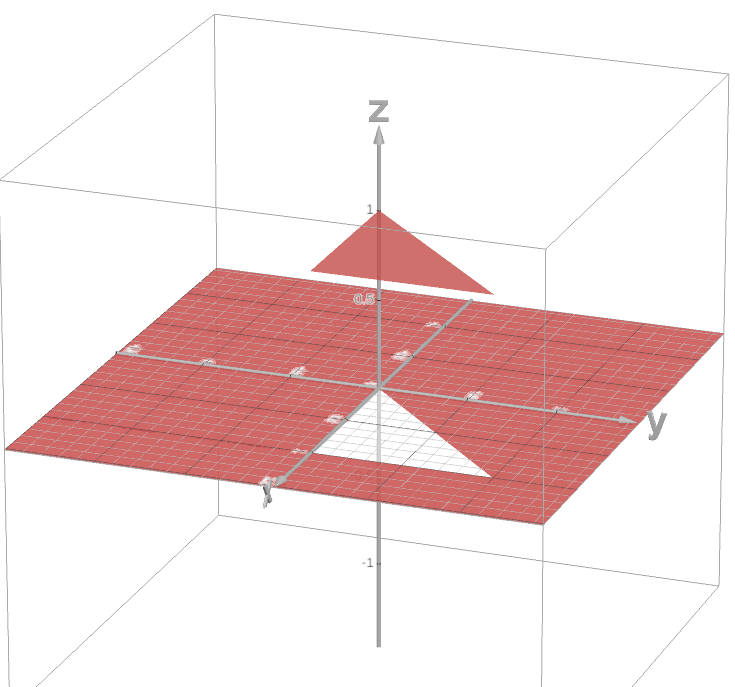
\includegraphics[scale=0.3]{figure1.png}
            \end{center}
        \item After some calculations, we get
            \[
                f_X (x) = \left\lbrace \begin{matrix} x & 0 \leq x \leq 1 \\ 0 & \text{elsewhere.} \end{matrix} \right.
            \]
        and
            \[
                f_Y (y) = \left\lbrace \begin{matrix} 1 - y & 0 \leq y \leq 1 \\ 0 & \text{elsewhere.} \end{matrix} \right. 
            \]
        We see that $f_{X, Y} (x, y) \neq f_X (x) f_Y (y)$ and therefore $X$ and $Y$ are dependent. \hfill $\square$
    \end{enumerate}
\end{problem}

\begin{problem}
    \begin{enumerate}[label=\alph*)]
        \item Below is a sketch of the density function using Desmos.
            \begin{center}
            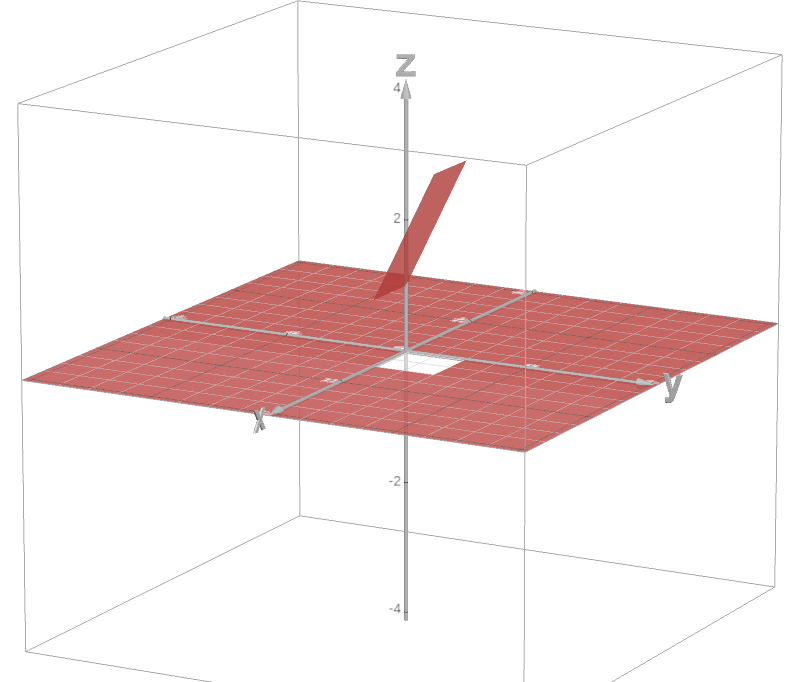
\includegraphics[scale=0.3]{figure2.png}
            \end{center}
        \item After some calculations, we get
            \[
                f_X (x) = \left\lbrace \begin{matrix} 1 & 0 \leq x \leq 1 \\ 0 & \text{elsewhere.} \end{matrix} \right.
            \]
        and
            \[
                f_Y (y) = \left\lbrace \begin{matrix} y + 1/2 & 0 \leq y \leq 1 \\ 0 & \text{elsewhere.} \end{matrix} \right. 
            \]
        We see that $f_{X, Y} (x, y) = f_X (x) f_Y (y)$ and therefore $X$ and $Y$ are independent. \hfill $\square$
    \end{enumerate}
\end{problem}

\begin{problem}
Let $X$ be the time of arrival of the passenger and let $Y$ be the time of arrival of the bus. We have $0 \leq X \leq 60$ and $0 \leq Y \leq 60$. Also, $X , Y \sim U (0, 60)$. Since there are independent, their joint density function is 
    \[
        f_{X, Y} (x, y) = f_X (x) f_Y (y) = \left\lbrace \begin{matrix} \frac{1}{3600} & (x, y) \in [0, 1] \times [0, 1] \\ 0 & \text{elsewhere} . \end{matrix} \right. 
    \]
Let $a$ be the arrival time of the passenger at the bus station. Since the passenger waits 15min for a bus to arrive, the bus must stops at the bus station between $a$min and $(a + 15)$min. Therefore, the probability is
    \[
        P (a \leq X \leq a + 15 , a \leq Y \leq a + 15 ) = \frac{15 \cdot 15}{3600} = \frac{25}{400} = \frac{1}{16} = 0.0625 . \tag*{$\square$}
    \]
\end{problem}

%\subsection{Sums of Random Variables}

\subsection*{Important Measurements}

\begin{problem}
Since $X$ and $Y$ are independent, then
    \[
        \mathrm{Cov} (X, Y) = \mathrm{Exp} (X Y) - \mathrm{Exp} (X) \mathrm{Exp} (Y) = 0
    \]
because $\mathrm{Exp} (XY) = \mathrm{Exp} (X) \mathrm{Exp} (Y)$.
\end{problem}

\begin{problem}
In this case, we need the Cauchy Schwarz inequality:
    \[
        |\mathrm{Exp} (XY)| \leq \sqrt{\mathrm{Exp} (X^2)} \sqrt{\mathrm{Exp} (Y^2)} .
    \]
Using that, we see that
    \[
        |\mathrm{Cov} (X, Y)| = \mathrm{Exp} ( (X - \mu_X ) (Y- \mu_Y)) \leq \sqrt{\mathrm{Exp} ( (X-\mu_X)^2)} \sqrt{\mathrm{Exp} ( (Y - \mu_Y)^2)} = \sigma_X \sigma_Y .
    \]
Therefore,
    \[
        |\rho (X, Y) | = \left| \frac{\mathrm{Cov} (X, Y)}{\sigma_X \sigma_Y} \right| \leq 1 . \tag*{$\square$}.
    \]
\end{problem}

\begin{problem}
    \begin{enumerate}[label=\alph*)]
        \item By definition,
            \[
                \mathrm{Cov} (X, Y) = \mathrm{Exp} ( (X -\mu_X) (Y - \mu_Y)) = \mathrm{Exp} ( (Y- \mu_Y) (X - \mu_X )) = \mathrm{Cov} (Y, X) .
            \]
        \item By the formula of the variance,
            \begin{align*}
                \mathrm{Var} (aX + bY) &= \mathrm{Exp} ( (aX + bY)^2)) - (\mathrm{Exp} (aX + bY))^2 \\ 
                &= a^2 \mathrm{Exp} (X^2) + 2ab \mathrm{Exp} (XY) + b^2 \mathrm{Exp} (Y^2) - a^2\mu_X^2 - 2ab \mu_X \mu_Y - b^2 \mu_Y^2 \\ 
                &= a^2 (\mathrm{Exp} (X^2) - \mu_X^2) + b^2 (\mathrm{Exp} (Y^2) - \mu_Y^2) + 2ab (\mathrm{Exp} (XY) - \mu_X \mu_Y ) \\ 
                &= a^2 \mathrm{Var} (X) + b^2 \mathrm{Var} (Y) + 2ab \mathrm{Cov} (X, Y) . 
            \end{align*} 
        \item By definition,
            \[
                \mathrm{Cov} (X, X) = \mathrm{Exp} ( (X - \mu_X) (X - \mu_X )) = \mathrm{Var} (X) . \tag*{$\square$}
            \]
    \end{enumerate}
\end{problem}

\begin{problem}
    \begin{enumerate}[label=\alph*)]
            \item Since $\mathrm{Cov} (X, X) = \mathrm{Var} (X)$, we find that $\mathrm{Cov} (X, X) = 2$. 
            \item Since $\rho (X, Y) \in [-1, 1]$, we see that
                \[
                    \frac{\mathrm{Cov} (X, Y)}{\sigma_X \sigma_Y} \leq 1 \quad \Rightarrow \quad \mathrm{Cov} (X, Y) \leq (\sqrt{2}) (2\sqrt{2}) = 4 . \tag*{$\square$}
                \]
    \end{enumerate}
\end{problem}

\end{comment}